\documentclass[a4paper,titlepage]{article}
\usepackage[utf8]{inputenc}
\usepackage{fullpage}
\usepackage{indentfirst}
\usepackage[per-mode=symbol]{siunitx}
\usepackage{listings}
\usepackage{graphicx}
\usepackage{color}
\usepackage{amsmath}
\usepackage{mathtools}
\usepackage{array}
\usepackage[hidelinks]{hyperref}
\usepackage[format=plain,font=it]{caption}
\usepackage{subcaption}
\usepackage{standalone}
\usepackage[nottoc]{tocbibind}
\usepackage[noabbrev,capitalize,nameinlink]{cleveref}
\usepackage{listings}
\usepackage{xspace}
\usepackage{tikz}
\usepackage{circuitikz}
\usepackage{titlesec}
\usepackage[cache=false]{minted}
\usepackage{booktabs}
\usepackage{csvsimple}
\newcommand{\MATLAB}{\textsc{Matlab}\xspace}
\usepackage{siunitx}
\usepackage[super]{nth}
\usepackage[titletoc]{appendix}

% Custom commands
\newcommand\numberthis{\addtocounter{equation}{1}\tag{\theequation}}
\newcommand{\code}[1]{\texttt{#1}}
\newcolumntype{P}[1]{>{\centering\arraybackslash}p{#1}}

\tikzstyle{my help lines}=[gray,thick,dashed]

\setminted{linenos,breaklines,fontsize=auto}

%\titleformat*{\section}{\normalsize\bfseries}
%\titleformat*{\subsection}{\small\bfseries}
\renewcommand{\thesubsection}{\thesection.\alph{subsection}}
\providecommand*{\listingautorefname}{Listing}
\newcommand*{\Appendixautorefname}{Appendix}

%opening
\title{\textbf{ECSE 543: Numerical Methods} \\ Assignment 2 Report}
\author{Wenjie Wei \\ 260685967}
\date{\today}

\begin{document}
	\sloppy
	\maketitle
	
	\tableofcontents
	\newpage
	
	\section*{Introduction}
		In this assignment, triangular finite element and conjugate gradient methods discussed in class were explored. The interpreter used for the Python codes is Python 3.6. 
		
	\section{First Order Finite Element Problem}
		Figure \ref{prob} shows an illustration of the first order triangular finite element problem to be solved. 
		\begin{figure}[!h]
			\centering
			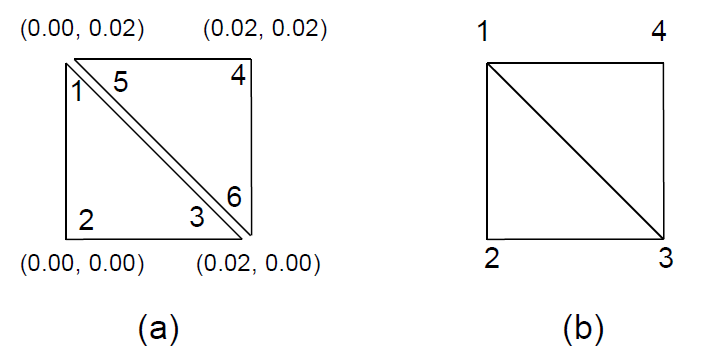
\includegraphics[width=0.7\linewidth]{prob}
			\caption{1st Order Triangular FE Problem}
			\label{prob}
		\end{figure}
	
		Take the triangle with nodes 1, 2, and 3 as the beginning step. Firstly, interpolate the potential \textit{U} as:
		$$
			U = a + bx + cy
		$$
		and at vertex 1, we can write an equation of potential as:
		$$
			U_1 = a + bx_1 + cy_1
		$$
		
		Thus, we can have a vector of potentials for vertex 1, 2, and 3 as follows:
		$$
			\begin{bmatrix}
				U_1 \\ U_2 \\ U_3
			\end{bmatrix} = 
			\begin{bmatrix}
				1 & x_1 & y_1 \\
				1 & x_2 & y_2 \\
				1 & x_3 & y_3 
			\end{bmatrix}
			\begin{bmatrix}
				a \\ b \\ c
			\end{bmatrix}
		$$
		and the terms $a, b, c$ are acquired following:
		\begin{equation}
			U = \sum_{i = 1}^{3} U_i\alpha_i(x, y)
		\end{equation}
		and we can derive a general formula for $\alpha_i$:
		\begin{equation}
			\nabla \alpha_i = \nabla \frac{1}{2A}[(x_{i+1}y_{i+2}-x_{i+2}y_{i+1}) + (y_{i+1}-y_{i+2})x+(x_{i+2}-x_{i+1})y]			
		\end{equation}
		where $A$ holds the value of the area of the triangle.
		
		Following Equation 2, when the index $i$ exceeds the top limit 3, it is wrapped around to 1. Now we can get the following calculations for $\alpha_1$, $\alpha_2$ and $\alpha_3$:
		$$
			\nabla \alpha_1 = \nabla \frac{1}{2A}[(x_2y_3-x_3y_2) + (y_2-y_3)x+(x_3-x_2)y]
		$$
		$$
			\nabla \alpha_2 = \nabla \frac{1}{2A}[(x_3y_1-x_1y_3) + (y_3-y_1)x+(x_1-x_3)y]
		$$
		$$
			\nabla \alpha_3 = \nabla \frac{1}{2A}[(x_1y_2-x_2y_1) + (y_1-y_2)x+(x_2-x_1)y]
		$$
		
		With the expressions for $\alpha$ derived, we now go ahead and calculate the \textbf{$S_{ij}^{(e)}$} matrices. The general formula below is used to calculate the \textbf{\textit{S}} matrix:
		\begin{equation}
			S^{(e)}_{ij} = \int_{\Delta e} \nabla \alpha_i \nabla \alpha_j dS
		\end{equation}
		
		Using the equation above, plug in the values provided in Figure \ref{prob}, we can have the following calculations:
		$$
			S_{11} = \frac{1}{4A}[(y_2 - y_3)^2 + (x_3 - x_2)^2] = \frac{1}{4 \times 2 \times 10^{-4}}[0 + 0.02^2] = 0.5
		$$
		$$
			S_{12} = \frac{1}{4A}[(y_2 - y_3)(y_3 - y_1) + (x_3 - x_2)(x_1 - x_3)] = -0.5
		$$
		$$
			S_{13} = \frac{1}{4A}[(y_2 - y_3)(y_1 - y_2) + (x_3 - x_2)(x_2 - x_1)] = 0
		$$
		
		Before performing the calculation for the next row, we inspect the calculation rules of the entries of the \textbf{\textit{S}} matrix, we can easily discover that $S_{ij} = S_{ji}$, since the flip of the orders of the operands in the parenthesis results in the same sign of the result. Therefore, the following statements can be made:
		$$
			S_{21} = S_{12} = -0.5
		$$
		$$
			S_{31} = S_{13} = 0
		$$
		
		$$
			S_{22} = \frac{1}{4A}[(y_3 - y_1)^2 + (x_1 - x_3)^2] = 1
		$$
		$$
			S_{23} = S_{32} = \frac{1}{4A}[(y_3 - y_1)(y_1 - y_2) + (x_1 - x_3)(x_2 - x_1)] = -0.5
		$$
		$$
			S_{33} = \frac{1}{4A}[(y_1 - y_2)^2 + (x_2 - x_1)^2] = 0.5
		$$
		
		From the calculation results above, we can come up with the \textbf{\textit{S}} matrix for vertices 1, 2, and 3:
		$$
			S^{(1)} = \begin{bmatrix}
				S_{11} & S_{12} & S_{13}\\
				S_{21} & S_{22} & S_{23} \\
				S_{31} & S_{32} & S_{33} \\
			\end{bmatrix} = 
			\begin{bmatrix}
				0.5 & -0.5 & 0\\
				-0.5 & 1 & -0.5 \\
				0 & -0.5 & 0.5
			\end{bmatrix}
		$$
		
		Use the similar approach for the other triangle and obtain $S_{456}$:
		$$
			S^{(2)} = \begin{bmatrix}
				S_{44} & S_{45} & S_{46}\\
				S_{54} & S_{55} & S_{56} \\
				S_{64} & S_{65} & S_{66} \\
			\end{bmatrix} = 
			\begin{bmatrix}
				1 & -0.5 & -0.5\\
				-0.5 & 0.5 & 0 \\
				-0.5 & 0 & 0.5
			\end{bmatrix}
		$$
		
		Add the triangles to get the energy of the whole system shown in (b) of Figure \ref{prob}:
		$$
			\begin{bmatrix}
				U_1 \\
				U_2 \\
				U_3 \\
				U_4 \\
				U_5 \\
				U_6				
			\end{bmatrix}_{dis} = 
			\begin{bmatrix}
				1&&&\\
				&1&&\\
				&&1&\\
				&&&1\\
				1&&&\\
				&&1&
			\end{bmatrix}
			\begin{bmatrix}
				U_1 \\
				U_2 \\
				U_3 \\
				U_4
			\end{bmatrix}_{joint}
		$$
		which is also denoted as:
		$$
			U_{dis} = CU_{joint}
		$$
		
		Use $\textbf{S}_{dis}$ to denote a $6\times 6$ matrix to represent the disjoint matrix:
		$$
			S_{dis} = 
			\begin{bmatrix}
				S^{(1)} & \\
				 & S^{(2)}				
			\end{bmatrix} = 
			\begin{bmatrix}
				0.5 & -0.5 & 0 & & & \\
				-0.5 & 1 & -0.5 & & & \\
				0 & -0.5 & 0.5 & & & \\
				& & & 1 & -0.5 & -0.5 \\
				& & & -0.5 & 0.5 & 0 \\
				& & & -0.5 & 0 & 0.5
			\end{bmatrix}
		$$
		
		Now the global \textbf{\textit{S}} matrix will be calculated as:
		\begin{align*}
			S_{joint} &= C^TS_{dis}C \\
			&= 
			\begin{bmatrix}
				1&&&&1&\\
				&1&&&&\\
				&&1&&&1\\
				&&&1&&
			\end{bmatrix}
			\begin{bmatrix}
				0.5 & -0.5 & 0 & & & \\
				-0.5 & 1 & -0.5 & & & \\
				0 & -0.5 & 0.5 & & & \\
				& & & 1 & -0.5 & -0.5 \\
				& & & -0.5 & 0.5 & 0 \\
				& & & -0.5 & 0 & 0.5
			\end{bmatrix}
			\begin{bmatrix}
				1&&&\\
				&1&&\\
				&&1&\\
				&&&1\\
				1&&&\\
				&&1&
			\end{bmatrix}\\
			&= \begin{bmatrix}
				1 & -0.5 & 0 & -0.5\\
				-0.5 & 1 & -0.5 & 0\\
				0 & -0.5 & 1 & -0.5\\
				-0.5 & 0 & -0.5 & 1
			\end{bmatrix}
		\end{align*}
		which is the final result of this problem.
	\section{Coaxial Cable Electrostatic Problem}
		Use the triangular finite element model for the analysis of the coaxial cable problem seen in the previous assignment. We take the third quadrant for the analysis. 
		\subsection{The Finite Element Mesh}
			Listing \ref{lst:finite_element} shows the implementation of the construction of the finite element mesh and the creation of the \MATLAB input file.
			\begin{figure}[!h]
				\centering
				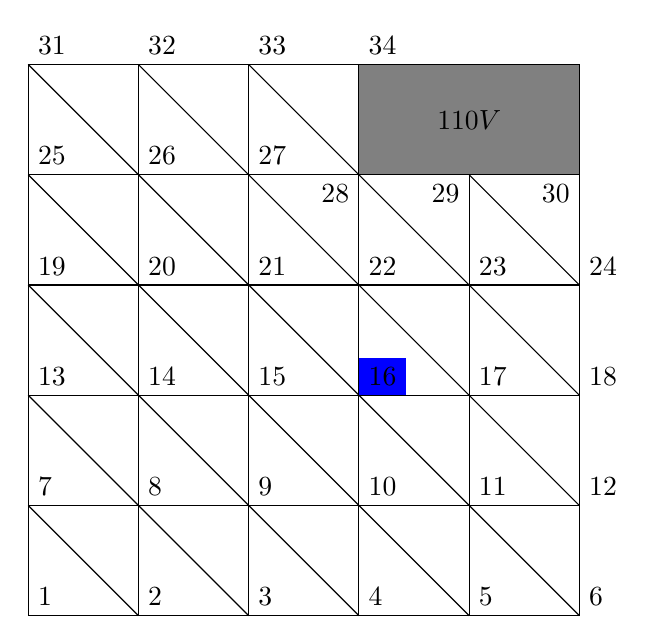
\begin{tikzpicture}[scale=1.4]
					\draw (0, 0) grid (5, 4);
					\draw (0,1) -- (1,0);
					\draw (0,2) -- (2,0);
					\draw (0,3) -- (3,0);
					\draw (0,4) -- (4,0);
					\draw (0,4) grid (3,5);
					\draw (0,5) -- (5,0);
					\draw (1,5) -- (5,1);
					\draw (2,5) -- (5,2);
					\draw (4,4) -- (5,3);
					\draw [fill=gray] (3,4) rectangle (5,5);					
					\node at (4, 4.5) {$110V$};
					\node[above right] at (0,0) {$1$};
					\node[above right] at (1,0) {$2$};
					\node[above right] at (2,0) {$3$};
					\node[above right] at (3,0) {$4$};
					\node[above right] at (4,0) {$5$};
					\node[above right] at (5,0) {$6$};
					\node[above right] at (0,1) {$7$};
					\node[above right] at (1,1) {$8$};
					\node[above right] at (2,1) {$9$};
					\node[above right] at (3,1) {$10$};
					\node[above right] at (4,1) {$11$};
					\node[above right] at (5,1) {$12$};
					\node[above right] at (0,2) {$13$};
					\node[above right] at (1,2) {$14$};
					\node[above right] at (2,2) {$15$};
					\node[fill=blue,above right] at (3,2) {$16$};
					
					\node[above right] at (4,2) {$17$};
					\node[above right] at (5,2) {$18$};
					\node[above right] at (0,3) {$19$};
					\node[above right] at (1,3) {$20$};
					\node[above right] at (2,3) {$21$};
					\node[above right] at (3,3) {$22$};
					\node[above right] at (4,3) {$23$};
					\node[above right] at (5,3) {$24$};
					\node[above right] at (0,4) {$25$};
					\node[above right] at (1,4) {$26$};
					\node[above right] at (2,4) {$27$};
					\node[below left] at (3,4) {$28$};
					\node[below left] at (4,4) {$29$};
					\node[below left] at (5,4) {$30$};
					\node[above right] at (0,5) {$31$};
					\node[above right] at (1,5) {$32$};
					\node[above right] at (2,5) {$33$};
					\node[above right] at (3,5) {$34$};
				\end{tikzpicture}
				\caption{Organization of the Finite Element Mesh}
				\label{fe_mesh_fig}
			\end{figure}
		
			Figure \ref{fe_mesh_fig} shows the organization of the finite element mesh constructed by the program. The input file written by this program is shown in Listing \ref{lst:SIMPLE2D.dat}. Note that the first number at the beginning of the lines are not an input to the \MATLAB file, as it is the line number which is provided by the \textit{minted} package in \LaTeX. 
			
		\subsection{Potential Solved by SIMPLE2D.m}
			Use the input file generated in the previous section, we are able to use the \MATLAB file to calculate the potential at every node we have specified. The output of the SIMPLE2D.m file is shown in Listing \ref{lst:potential.dat}. The target node (0.06, 0.04) is highlighted in blue as Node 16, and from Listing \ref{lst:potential.dat} shows that the potential at this node is $40.527V$.
			
		\subsection{Capacitance per Unit Length}\label{find_capacitance}
			To compute the capacitance, apply the fundamental Equation \ref{capacitance}: 
			\begin{equation}
				E = \frac{1}{2} CV^2
				\label{capacitance}
			\end{equation}
			
			Now apply the finite element method used in the previous section. Use $U_{joint}$ to denote the potential vector shown in Listing \ref{lst:potential.dat}. Use the $S_{joint}$ calculated in the first question, we derive an equation to calculate the energy for each square finite element:
			\begin{equation}
				W = \frac{1}{2}U^T_{joint}S_{joint}U_{joint}
				\label{USU}
			\end{equation}
			
			The value of the entries in the $U$ matrix are the potential on the four corners of the square defined by the two finite element triangles.
			
			Use the Python function implemented in Listing \ref{lst:finite_element} which applies Equation \ref{USU}, we are able to calculate the total energy contained in the cable. The calculation for the energy and capacitance is shown in Figure \ref{q2_run}.
			\begin{figure}[!h]
				\centering
				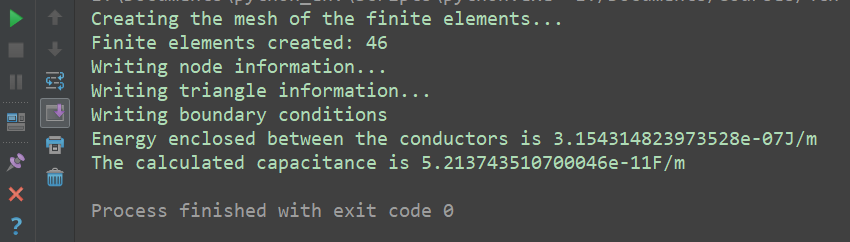
\includegraphics[width=0.7\linewidth]{q2_run}
				\caption{Running Results of $finite\_element.py$}
				\label{q2_run}
			\end{figure}
			
			The energy contained in the cable per unit length is calculated to be $3.154\times 10^{-7}J/m$. The following calculation is performed to find the total capacitance per unit length:
			$$
				C = \frac{2E}{V^2} = \frac{2\varepsilon_0 W}{V^2} = 5.2137\times 10^{-11}F/m
			$$
			which equals to $52.137pF/m$.
			
		\section{Conjugate Gradient}
			Listing \ref{lst:conjugate_gradient} shows the implementation of the conjugate gradient method. The important step of this problem is to find the matrix \textbf{\textit{A}} and the vector $\vec{b}$ to form the equation
			$$
				A\vec{x} = \vec{b}
			$$
			to perform Choleski decomposition and conjugate gradient.
			
			For this particular problem, since the Laplace's equation
			\begin{equation}
				\nabla ^2V = 0
			\end{equation}
			holds for every free node, the matrix equation
			$$
				\textbf{A}\vec{v} = 0
			$$
			is a valid assumption. Therefore, we may fill up the $\vec{b}$ with 0 and $-110V$, to the nearest free node of the Dirichlet nodes, which results in a $\vec{b}^T$ shown in Figure \ref{v_T}.
			\begin{figure}[!h]
				\centering
				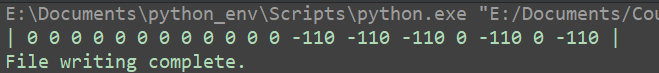
\includegraphics[width=0.7\linewidth]{v_T}
				\caption{Initialized $\vec{b}^T$ vector}
				\label{v_T}
			\end{figure}
		
			With the matrices and vectors generated, we may proceed and calculate the potential at every node of this system using Choleski decomposition and conjugate gradient. 
			
			\subsection{S. P. D. Check}
				Use the Choleski decomposition implemented in the previous assignment and check if the matrix \textbf{\textit{A}} is symmetric, positive definite. The program fails with an exception when performing the symmetry check. Moreover, by inspection of the diagonal, it is obvious that the matrix is not positive definite. Therefore, the matrix \textit{\textbf{A}} is not symmetric, positive definite. 
				
				To obtain a symmetric, positive definite matrix in order to pass the Choleski decomposition test, we multiply the transpose of matrix \textbf{\textit{A}} to both sides of the equation, obtaining:
				\begin{align*}
					A\vec{x} &= \vec{b}\\
					A^T \cdot A\vec{x} &= A^T\vec{b}
				\end{align*}
				
				$A^T \cdot A$ is proved to be symmetric, positive definite. This way, the Choleski decomposition succeeds. The result of the computations will be discussed in the following sections. 
			\subsection{Choleski and C.G. Results}	
				Table \ref{table:cg_result} shows the comparison between the computational results of Choleski decomposition and conjugate gradient.			
				\begin{table}[!htb]
					\centering
					\caption{Computational Results of Choleski Decomposition and Conjugate Gradient}
					\csvautobooktabular{../outputs/cg_result.csv}
					\label{table:cg_result}
				\end{table}
			
				The error tolerance of the conjugate gradient method is set to be $1\times 10^{-5}$. As can be seen from the table, the results returned by the two algorithms are very similar. There is a difference at the order of $10^{-10}$, which is small enough to neglect for this problem.
			\subsection{$\infty$ Norm and 2-Norm}
				\begin{figure}[H]
					\centering
					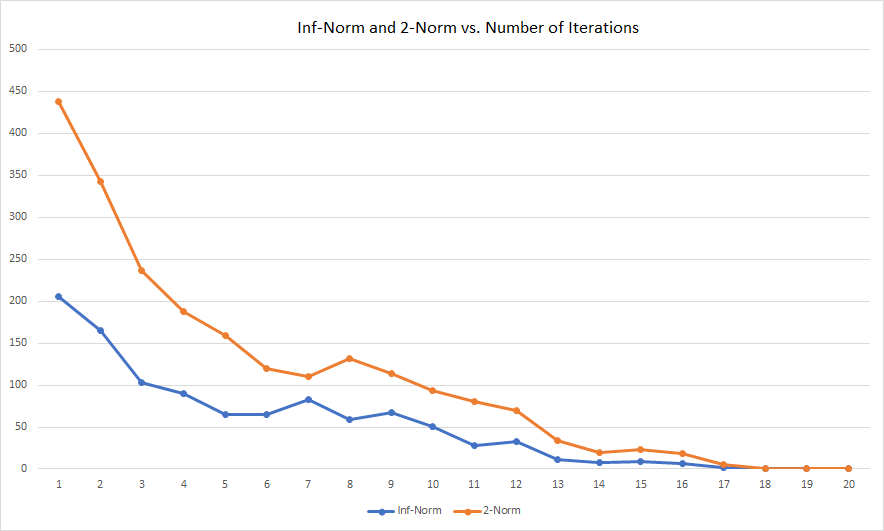
\includegraphics[width=0.7\linewidth]{two_norm_plot}
					\caption{Plot of $\infty$-norm and $2$-norm v.s. iterations}
					\label{two_norm_plot}
				\end{figure}	
				To calculate the $\infty$-norm and 2-norm of the residual vectors, we apply the following equations:
				\begin{equation}
					||r||_{\infty} = max(r_i)
				\end{equation}
				\begin{equation}
					||r||_2 = \sqrt{\sum_{i} |r_i|^2}
				\end{equation}
				
				Table \ref{table:norm} shows the $\infty$-norm and two-norm results of the conjugate gradient algorithm. Figure \ref{two_norm_plot} shows the $\infty$-norm and the two-norm plots with respect to the number of iterations. The orange line represents the two-norm curve and the blue line represents the $\infty$-norm curve. 
				\begin{table}[!htb]
					\centering
					\caption{$\infty$-Norm and two-Norm}
					\csvautobooktabular{../outputs/norm.csv}
					\label{table:norm}
				\end{table}
			\subsection{Potential at (0.06, 0.04)}
				From Table \ref{table:cg_result}, the potential at (0.06, 0.04) calculated by Choleski decomposition and conjugate gradient is 40.527$V$, which matches the result calculated in Section 2.b using SIMPLE2D.m.
				
				According to the results from the previous assignment, with $h = 0.02$, the potential calculated by SOR is 40.526$V$, which also matches the results calculated using the algorithms stated above. 
			\subsection{Computation of Capacitance per Unit Length}
				To compute the capacitance per unit length between the conductors, we go back and apply Equation \ref{capacitance} and transform it to the following form:
				$$
					C = \frac{2E}{V^2}
				$$
				
				Where $E$ is the electric field. The energy stored in the electric field is given by
				\begin{equation}
					U_E = \frac{\varepsilon_0}{2}\int \int (E_x^2 + E_y^2)dxdy
				\end{equation}
				
				Since we have already calculated the potential at every node, we can sum up the results and thus find the capacitance formed by the coaxial cable conductors.
				
				Alternatively, we could again use the finite element method discussed in Section \ref{find_capacitance} to find the capacitance per unit length.
				
	\newpage
	\begin{appendices}
		
		\section{Code Listings} \label{appendix:code}
		
		\setminted{linenos,breaklines,fontsize=\footnotesize}
		
		\begin{center}
			\captionof{listing}{Finite Element Mesh Implementation (\texttt{finite\_element.py}).}
			\inputminted{python}{../finite_element.py}
			\label{lst:finite_element}
		\end{center}
		
		\newpage
		\twocolumn
		\begin{center}
			\captionof{listing}{Finite Element Mesh Input File}
			\inputminted{python}{../SIMPLE2Dinput.dat}
			\label{lst:SIMPLE2D.dat}
		\end{center}
	
		\begin{center}
			\captionof{listing}{\MATLAB File Outputs}
			\inputminted{python}{../potentials.dat}
			\label{lst:potential.dat}
		\end{center}
		\newpage
		
		\onecolumn
		\begin{center}
			\captionof{listing}{Conjugate Gradient Implementation}
			\inputminted{python}{../conjugate_gradient.py}
			\label{lst:conjugate_gradient}
		\end{center}
		\begin{center}
			\captionof{listing}{Choleski Decompostition Implementation}
			\inputminted{python}{../choleski.py}
			\label{lst:chol}
		\end{center}
	\end{appendices}
	
\end{document}